% User verification
% - Biometria twarzy
% - Ogólna procedura weryfikacji 
% - Przetwarzanie wstępne 
% - Neuronowy extractor cech
%   * Klasyfikacja
%   * Triplet loss
%       - Negative examples sampling
% - Implementacja


\section[verification]{System weryfikacji użytkownika za pomocą biometrii twarzy}\label{sec:verification}

Kontrola dostępu, autoryzacja i identyfikacja osób jest wciąż otwartym problemem informatyki.
Implementacja polega zazwyczaj na podaniu przez osobę uwierzytelnianą kodu alfanumerycznego lub
zweryfikowaniu się kluczem(np. karta magnetyczna lub chipowa). Najbezpieczniejsze systemy
zabezpieczeń bazują jednak na cechach biometrycznych takie jak odcisk palca, tęczówka lub twarz.
Pomimo gorszej dokładności systemów bazujących na biometrii twarzy w porównaniu do innych, są one
bardzo często stosowane dzięki nieinwazyjności, bezkontaktowego dokonania pomiaru i popularności
w innych aplikacjach~\cite{FaceBiometric}.

\begin{figure}[h]
    \centering
    \includegraphics[width=1.\textwidth]{2-0_verification_general_drawio.pdf}
    \caption{\textbf{Proces weryfikacji użytkownika.} Proces rozpoczyna się od wykonania
    zdjęcia. Dalsze procesowanie składa się z etapu detekcji twarzy, wyznaczenia wektora cech twarzy(embeddingu) oraz porównania wektora z bazą danych.}
    \label{fig:proces_weryfikacji}
\end{figure}

Proces weryfikacji biometrią twarzy został pokazany na rysunku~\ref{fig:proces_weryfikacji}. Jak
w każdym innym tradycyjnym systemie kontroli dostępu potrzeba jest baza użytkowników. Tutaj dla
każdej z autoryzowanych osób przechowuje się wektor z wyznaczonymi cechami jej twarzy.
Wyznaczanie wektora zależy od zastosowanej metody i zostanie to omówione w
sekcji~\ref{sec:ekstraktor}. System na wejściu przyjmuje zdjęcie osoby poddawanej weryfikacji.
Technika wykonania zdjęcia zależy od realizacji systemu wizyjnego dlatego musi ono zostać
wstępnie przetworzone - usuwane jest zbędne tło i jest ono normalizowane(sekcja~\ref{sec:ekstrakcja_twarzy}). Następnie, powstały w
poprzednim kroku thumbnail twarzy przekształcany jest do tej samej przestrzeni wektorowej, do
której zostały zamienione twarze w bazie referencyjnej. W ten sposób w kolejnym kroku możemy w
prosty sposób porównać te wektory i stwierdzić czy weryfikacja jest pozytywna lub negatywna co
zostało omówione w sekcji~\ref{sec:verify_process}.


\subsection{Ekstrakcja twarzy i normalizacja obrazu}\label{sec:ekstrakcja_twarzy}
Wstępne przetwarzanie obrazu jest koniecznym krokiem w większości systemach wykorzystujących
wizje. Na zdjęciu na wejściu systemu oprócz twarzy osoby weryfikowanej mogą znajdować się 
w tle również twarze innych osób, dlatego w tym przypadku niezbędne będzie wykorzystanie metod
detekcji twarzy oraz algorytmów ciasnego dopasowania zdjęcia do jej konturów. Pod uwagę były
brane dwie architektury - MTCNN oraz RetinaFace. Wybór został ograniczony do tych dwóch głównie
ze względu na ich popularność, dobrą wydajność oraz to, że realizują to zadanie w sposób
end-to-end. Obie sieci z obrazu wejściowego wyekstrahują obszary, na których znajdują się twarze
i zwracają tę informację w postaci wektorów reprezentujących prostokąt na płaszczyźnie obrazu, w
którym znajduje się ciasno dopasowana twarz. Ze wszystkich twarzy wybierana jest ta, której
prostokąt ma największe pole - zakładamy, że użytkownik weryfikujący się znajduję się najbliżej
obiektywu kamery przez co jego twarz powinna być największa.

W tabeli~\ref{table:face_detector} pokazano porównanie dwóch detektorów twarzy. Z uwagi na to, że
ostatecznie największe znaczenie dla użytkownika końcowego ma dokładność całego systemu
porównujemy tutaj właśnie dokładność weryfikacji z wykorzystaniem ArcFace~\cite{Arcface} na
zbiorze danych LFW~\cite{DatasetLFW} w zależności od zastosowanego detektora twarzy. Wybrany
metoda będzie pracowała na urządzeniu o IoT dlatego porównujemy również szybkość modeli i 
rozmiar zapisanych wag na dysku. Czas inferencji jest średnim czasem jaki potrzebuje sieć na
przetworzenie jednego zdjęcia o rozdzielczości 320x240 pikseli. Uśredniona została detekcja na
wszystkich zdjęciach z zbioru LWF. Pomiary były wykonywane na urządzeniu RaspberryPi 4b
wykorzystując wszystkie dostępne rdzenie procesora.

\begin{table}[h]
\begin{center}
\begin{tabular}{cccc}
\hline
model & dokładność weryfikacji (\%)  &  czas inferencji (ms)  &   rozmiar na dysku (MB)  \\
\hline
MTCNN \cite{MTCNN}     & \num{99.83} & \num{83} & \num{1.9} \\ 
RetinaFace \cite{RetinaFace}   & \num{99.86}  & \num{112}& \num{1.8}  \\
\hline
\end{tabular}
\end{center}
\caption{\textbf{Porównanie detektorów twarzy}.}
\label{table:face_detector}
\vspace{-4mm}
\end{table}

W dalszej części pracy zostanie wykorzystany ekstraktor MTCC. Wybrano go głównie ze względu na jego
powszechność zastosowania w neuronowych metodach weryfikacji~\cite{Cosface,Arcface,Facenet}, szybkość oraz wystarczającą dokładność i wielkość na dysku. Na rysunku \ref{fig:ekstraktor_twarzy}
pokazano działanie wybranej architektury na przykładowych zdjęciach znajdujących sie w zbiorze
LFW. W celu analizy błędów jakie popełnia wybrany algorytm zostały pokazane
również przykłądy zdjęć z niewłaściwą detekcją - twarz została poprawnie wykryta ale nie jest ona
tą konkretną twarzą otagowaną w zbiorze danych. Obrazy te pokazują, że o ile zdjęcie zostanie wykonane w sposób właściwy, to jest, twarz osoby weryfikującej się będzie zajmowała największą część zdjęcia to błędy detektora nie powinny się propagować i wpływać na ostateczną wydajność weryfikacji.

\begin{figure}[H]
    \begin{center}
    \renewcommand\tabcolsep{1pt}
    {\bf Poprawna detekcja}
    \begin{tabular}{cc||cc||cc}
      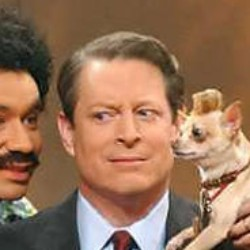
\includegraphics[width=.15\linewidth]{img/crop_examples/before/good/Al_Gore_0007.jpg} &
      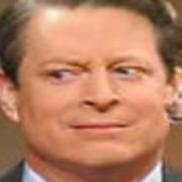
\includegraphics[width=.15\linewidth]{img/crop_examples/after/good/Al_Gore_0007.jpg} &
      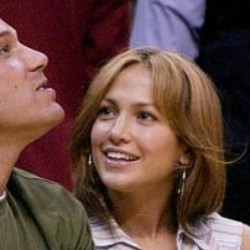
\includegraphics[width=.15\linewidth]{img/crop_examples/before/good/Jennifer_Lopez_0021.jpg} &
      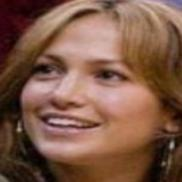
\includegraphics[width=.15\linewidth]{img/crop_examples/after/good/Jennifer_Lopez_0021.jpg} &
      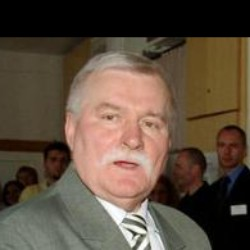
\includegraphics[width=.15\linewidth]{img/crop_examples/before/good/Lech_Walesa_0002.jpg} &
      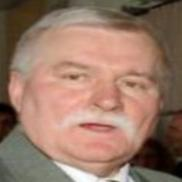
\includegraphics[width=.15\linewidth]{img/crop_examples/after/good/Lech_Walesa_0002.jpg} \\
    \end{tabular}
    {\bf Niepoprawna detekcja}
    \begin{tabular}{cc||cc||cc}
      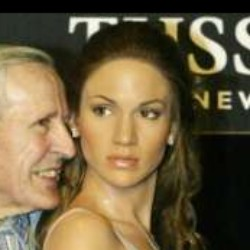
\includegraphics[width=.15\linewidth]{img/crop_examples/before/bad/Jennifer_Lopez_0020.jpg} &
      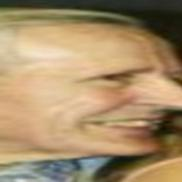
\includegraphics[width=.15\linewidth]{img/crop_examples/after/bad/Jennifer_Lopez_0020.jpg} &
      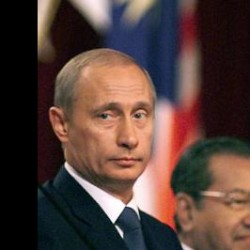
\includegraphics[width=.15\linewidth]{img/crop_examples/before/bad/Vladimir_Putin_0031.jpg} &
      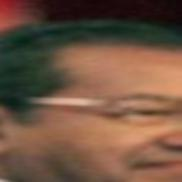
\includegraphics[width=.15\linewidth]{img/crop_examples/after/bad/Vladimir_Putin_0031.jpg} &
      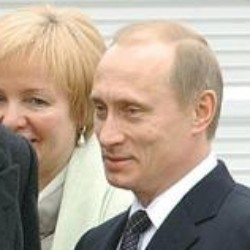
\includegraphics[width=.15\linewidth]{img/crop_examples/before/bad/Vladimir_Putin_0040.jpg} &
      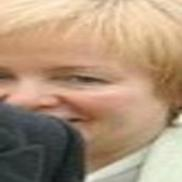
\includegraphics[width=.15\linewidth]{img/crop_examples/after/bad/Vladimir_Putin_0040.jpg} \\
    \end{tabular}
    \end{center}
    \caption{{\bf Przykłady działania ekstraktora twarzy.} Pokazane zostały tutaj wybrane przykłady prezentujące działanie ekstraktora twarzy.}
    \label{fig:ekstraktor_twarzy}
    \end{figure}

\subsection{Neuronowy ekstraktor cech} \label{sec:ekstraktor}

We współczesnych systemach weryfikacji wykorzystuje się głębokie sieci konwolucyjne. W
szczegółach zostaną omówione używana przez nas architektura w sekcji XXX. Pomijając szczegóły
modelu i traktując go jako czarną skrzynkę ogólna idea ekstraktora została pokazana na Rysunku
\ref{fig:ekstraktor_cech}. Głównym założeniem jest stworzenie systemu end-to-end, którego
rezultatem działania będzie embedding \(f(x)\), wyznaczony z obrazu wejściowego \(x\) przez
rzutowanie go do pewnej przestrzeni cech \(\mathbb{R}^d\), w taki sposób, że pewna funkcja
odległości wyznaczona dla wszystkich zdjęć twarzy jest mała dla twarzy należących do tych samych
osób i duża dla różnych twarzy. 

\begin{figure}[h]
    \centering
    \includegraphics[width=0.75\textwidth]{2-0_verification_ekstraktor_cech_drawio.pdf}
    \caption{\textbf{Struktura ekstraktora cech.} Ekstraktor składa się z wejścia, które w ogólnym przypadku może być paczką \(B\) przetworzonych wstępnie obrazów twarzy o wymiarach \( W \times H \times C\), głębokiej sieci konwolucyjnej i następującej po niej warstwie normalizacji. W rezultacie na wyjściu otrzymujemy \(B\) wektorów cech o wymiarach \(D\).}
    \label{fig:ekstraktor_cech}
\end{figure}


W literaturze można znaleźć dwie rodziny algorytmów trenujących, jedna wzorująca się na
klasycznym podejściu stosowanym podczas treningu klasyfikatorów obrazów. Najnowsze podejścia z
tej rodziny algorytmów prezentujemy w sekcji \ref{sec:klasyfikatory}. Drugi rodzaj algorytmów
bazują na optymalizacji multi-class classification hinge loss (po pl?). Opisujemy je w
szczegółach w sekcji \ref{sec:tripletloss}

\subsubsection{Klasyfikacja twarzy}\label{sec:klasyfikatory}
\begin{figure}[h!]
\centering
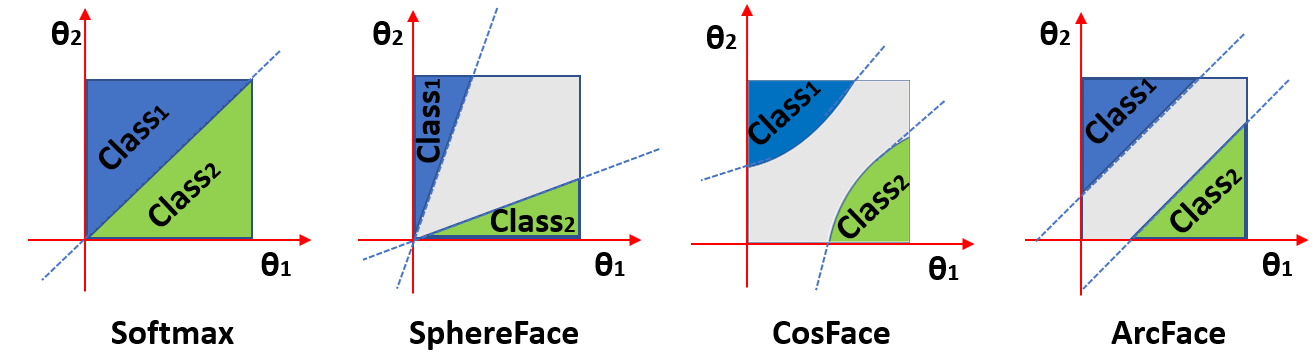
\includegraphics[width=1\linewidth]{img/margincompare.png}
\caption{Porównanie marginesów decyzyjnych\cite{}}
\vspace{-4mm}
\label{fig:binarymargin}
\end{figure}
\paragraph{Softmax\cite{Centreloss}}
\paragraph{SphereFace}
\paragraph{CosFace\cite{Cosface}}
\paragraph{ArcFace\cite{Arcface}}


\subsubsection{FaceNet}\label{sec:tripletloss}
% \begin{align}\label{eq:triplet_dystant}
    % \left\Vert f(x_i) - f(x_j) \right\Vert_q^p < \alpha
% \end{align}


\subsection{Procedura weryfikacji przy wykorzystaniu sieci neuronowych}\label{sec:verify_process}

Weryfikacja twarzy jest zadaniem przyrównania twarzy kandydata 
do innej i sprawdzenie czy nastąpiło ich dopasowanie. Jest to mapowanie
jeden-do-jednego: należy sprawdzić czy jest to ta sama osoba.

Mając na wejściu systemu dwa zdjęcia \(x_i\) oraz \(x_j\) wynik weryfikacji będzie wyznaczany następująco:

\begin{align}\label{eq:ekstraktor_weryfikacja}
\text{weryfikacja jest}\begin{cases}
    \text{pozytywna},& \text{jeśli } d(f(x_i), f(x_j) < \alpha \\
    \text{negatywna},              & \text{w.p.p}
\end{cases}
\end{align}

gdzie \(f(x)\) jest wektorem cech obrazu \(x\), opisanym w sekcji
\ref{sec:ekstraktor}, \(\alpha\) jest marginesem, \(d(f_1, f_2)\) jest pewną funkcją dystansu liczoną pomiędzy wektorami wyznaczanymi przez \(f(x)\).
